% This file was created by matplotlib2tikz v0.6.13.
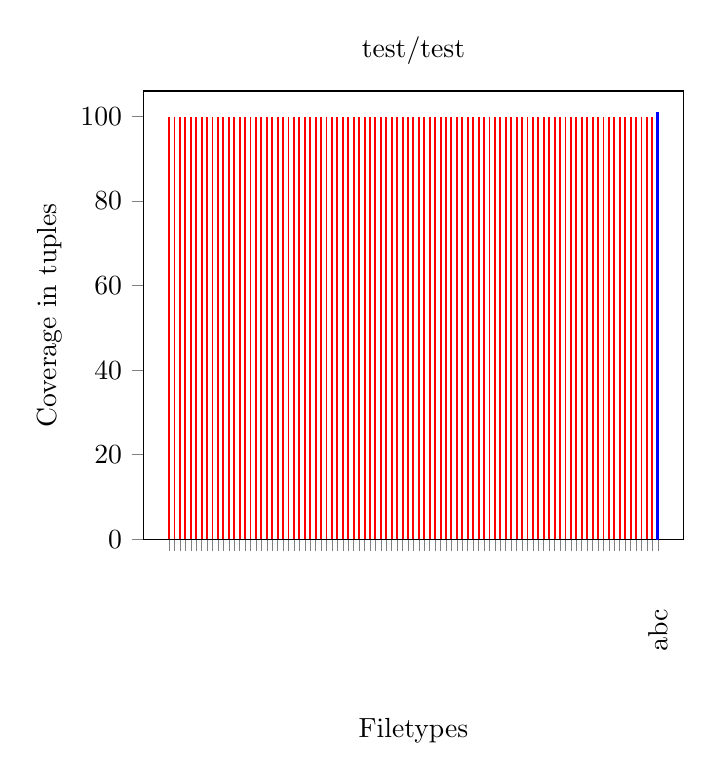
\begin{tikzpicture}

\begin{axis}[
title={test/test},
xlabel={Filetypes},
ylabel={Coverage in tuples},
xmin=-4.6925, xmax=94.6925,
ymin=0, ymax=106.05,
xtick={0,1,2,3,4,5,6,7,8,9,10,11,12,13,14,15,16,17,18,19,20,21,22,23,24,25,26,27,28,29,30,31,32,33,34,35,36,37,38,39,40,41,42,43,44,45,46,47,48,49,50,51,52,53,54,55,56,57,58,59,60,61,62,63,64,65,66,67,68,69,70,71,72,73,74,75,76,77,78,79,80,81,82,83,84,85,86,87,88,89,90},
xticklabels={,,,,,,,,,,,,,,,,,,,,,,,,,,,,,,,,,,,,,,,,,,,,,,,,,,,,,,,,,,,,,,,,,,,,,,,,,,,,,,,,,,,,,,,,,,abc},
tick align=outside,
xticklabel style = {rotate=90,align=center,text width=50},
tick pos=left,
x grid style={white!69.019607843137251!black},
y grid style={white!69.019607843137251!black}
]
\draw[fill=red,draw opacity=0] (axis cs:-0.175,0) rectangle (axis cs:0.175,100);
\draw[fill=red,draw opacity=0] (axis cs:0.825,0) rectangle (axis cs:1.175,100);
\draw[fill=red,draw opacity=0] (axis cs:1.825,0) rectangle (axis cs:2.175,100);
\draw[fill=red,draw opacity=0] (axis cs:2.825,0) rectangle (axis cs:3.175,100);
\draw[fill=red,draw opacity=0] (axis cs:3.825,0) rectangle (axis cs:4.175,100);
\draw[fill=red,draw opacity=0] (axis cs:4.825,0) rectangle (axis cs:5.175,100);
\draw[fill=red,draw opacity=0] (axis cs:5.825,0) rectangle (axis cs:6.175,100);
\draw[fill=red,draw opacity=0] (axis cs:6.825,0) rectangle (axis cs:7.175,100);
\draw[fill=red,draw opacity=0] (axis cs:7.825,0) rectangle (axis cs:8.175,100);
\draw[fill=red,draw opacity=0] (axis cs:8.825,0) rectangle (axis cs:9.175,100);
\draw[fill=red,draw opacity=0] (axis cs:9.825,0) rectangle (axis cs:10.175,100);
\draw[fill=red,draw opacity=0] (axis cs:10.825,0) rectangle (axis cs:11.175,100);
\draw[fill=red,draw opacity=0] (axis cs:11.825,0) rectangle (axis cs:12.175,100);
\draw[fill=red,draw opacity=0] (axis cs:12.825,0) rectangle (axis cs:13.175,100);
\draw[fill=red,draw opacity=0] (axis cs:13.825,0) rectangle (axis cs:14.175,100);
\draw[fill=red,draw opacity=0] (axis cs:14.825,0) rectangle (axis cs:15.175,100);
\draw[fill=red,draw opacity=0] (axis cs:15.825,0) rectangle (axis cs:16.175,100);
\draw[fill=red,draw opacity=0] (axis cs:16.825,0) rectangle (axis cs:17.175,100);
\draw[fill=red,draw opacity=0] (axis cs:17.825,0) rectangle (axis cs:18.175,100);
\draw[fill=red,draw opacity=0] (axis cs:18.825,0) rectangle (axis cs:19.175,100);
\draw[fill=red,draw opacity=0] (axis cs:19.825,0) rectangle (axis cs:20.175,100);
\draw[fill=red,draw opacity=0] (axis cs:20.825,0) rectangle (axis cs:21.175,100);
\draw[fill=red,draw opacity=0] (axis cs:21.825,0) rectangle (axis cs:22.175,100);
\draw[fill=red,draw opacity=0] (axis cs:22.825,0) rectangle (axis cs:23.175,100);
\draw[fill=red,draw opacity=0] (axis cs:23.825,0) rectangle (axis cs:24.175,100);
\draw[fill=red,draw opacity=0] (axis cs:24.825,0) rectangle (axis cs:25.175,100);
\draw[fill=red,draw opacity=0] (axis cs:25.825,0) rectangle (axis cs:26.175,100);
\draw[fill=red,draw opacity=0] (axis cs:26.825,0) rectangle (axis cs:27.175,100);
\draw[fill=red,draw opacity=0] (axis cs:27.825,0) rectangle (axis cs:28.175,100);
\draw[fill=red,draw opacity=0] (axis cs:28.825,0) rectangle (axis cs:29.175,100);
\draw[fill=red,draw opacity=0] (axis cs:29.825,0) rectangle (axis cs:30.175,100);
\draw[fill=red,draw opacity=0] (axis cs:30.825,0) rectangle (axis cs:31.175,100);
\draw[fill=red,draw opacity=0] (axis cs:31.825,0) rectangle (axis cs:32.175,100);
\draw[fill=red,draw opacity=0] (axis cs:32.825,0) rectangle (axis cs:33.175,100);
\draw[fill=red,draw opacity=0] (axis cs:33.825,0) rectangle (axis cs:34.175,100);
\draw[fill=red,draw opacity=0] (axis cs:34.825,0) rectangle (axis cs:35.175,100);
\draw[fill=red,draw opacity=0] (axis cs:35.825,0) rectangle (axis cs:36.175,100);
\draw[fill=red,draw opacity=0] (axis cs:36.825,0) rectangle (axis cs:37.175,100);
\draw[fill=red,draw opacity=0] (axis cs:37.825,0) rectangle (axis cs:38.175,100);
\draw[fill=red,draw opacity=0] (axis cs:38.825,0) rectangle (axis cs:39.175,100);
\draw[fill=red,draw opacity=0] (axis cs:39.825,0) rectangle (axis cs:40.175,100);
\draw[fill=red,draw opacity=0] (axis cs:40.825,0) rectangle (axis cs:41.175,100);
\draw[fill=red,draw opacity=0] (axis cs:41.825,0) rectangle (axis cs:42.175,100);
\draw[fill=red,draw opacity=0] (axis cs:42.825,0) rectangle (axis cs:43.175,100);
\draw[fill=red,draw opacity=0] (axis cs:43.825,0) rectangle (axis cs:44.175,100);
\draw[fill=red,draw opacity=0] (axis cs:44.825,0) rectangle (axis cs:45.175,100);
\draw[fill=red,draw opacity=0] (axis cs:45.825,0) rectangle (axis cs:46.175,100);
\draw[fill=red,draw opacity=0] (axis cs:46.825,0) rectangle (axis cs:47.175,100);
\draw[fill=red,draw opacity=0] (axis cs:47.825,0) rectangle (axis cs:48.175,100);
\draw[fill=red,draw opacity=0] (axis cs:48.825,0) rectangle (axis cs:49.175,100);
\draw[fill=red,draw opacity=0] (axis cs:49.825,0) rectangle (axis cs:50.175,100);
\draw[fill=red,draw opacity=0] (axis cs:50.825,0) rectangle (axis cs:51.175,100);
\draw[fill=red,draw opacity=0] (axis cs:51.825,0) rectangle (axis cs:52.175,100);
\draw[fill=red,draw opacity=0] (axis cs:52.825,0) rectangle (axis cs:53.175,100);
\draw[fill=red,draw opacity=0] (axis cs:53.825,0) rectangle (axis cs:54.175,100);
\draw[fill=red,draw opacity=0] (axis cs:54.825,0) rectangle (axis cs:55.175,100);
\draw[fill=red,draw opacity=0] (axis cs:55.825,0) rectangle (axis cs:56.175,100);
\draw[fill=red,draw opacity=0] (axis cs:56.825,0) rectangle (axis cs:57.175,100);
\draw[fill=red,draw opacity=0] (axis cs:57.825,0) rectangle (axis cs:58.175,100);
\draw[fill=red,draw opacity=0] (axis cs:58.825,0) rectangle (axis cs:59.175,100);
\draw[fill=red,draw opacity=0] (axis cs:59.825,0) rectangle (axis cs:60.175,100);
\draw[fill=red,draw opacity=0] (axis cs:60.825,0) rectangle (axis cs:61.175,100);
\draw[fill=red,draw opacity=0] (axis cs:61.825,0) rectangle (axis cs:62.175,100);
\draw[fill=red,draw opacity=0] (axis cs:62.825,0) rectangle (axis cs:63.175,100);
\draw[fill=red,draw opacity=0] (axis cs:63.825,0) rectangle (axis cs:64.175,100);
\draw[fill=red,draw opacity=0] (axis cs:64.825,0) rectangle (axis cs:65.175,100);
\draw[fill=red,draw opacity=0] (axis cs:65.825,0) rectangle (axis cs:66.175,100);
\draw[fill=red,draw opacity=0] (axis cs:66.825,0) rectangle (axis cs:67.175,100);
\draw[fill=red,draw opacity=0] (axis cs:67.825,0) rectangle (axis cs:68.175,100);
\draw[fill=red,draw opacity=0] (axis cs:68.825,0) rectangle (axis cs:69.175,100);
\draw[fill=red,draw opacity=0] (axis cs:69.825,0) rectangle (axis cs:70.175,100);
\draw[fill=red,draw opacity=0] (axis cs:70.825,0) rectangle (axis cs:71.175,100);
\draw[fill=red,draw opacity=0] (axis cs:71.825,0) rectangle (axis cs:72.175,100);
\draw[fill=red,draw opacity=0] (axis cs:72.825,0) rectangle (axis cs:73.175,100);
\draw[fill=red,draw opacity=0] (axis cs:73.825,0) rectangle (axis cs:74.175,100);
\draw[fill=red,draw opacity=0] (axis cs:74.825,0) rectangle (axis cs:75.175,100);
\draw[fill=red,draw opacity=0] (axis cs:75.825,0) rectangle (axis cs:76.175,100);
\draw[fill=red,draw opacity=0] (axis cs:76.825,0) rectangle (axis cs:77.175,100);
\draw[fill=red,draw opacity=0] (axis cs:77.825,0) rectangle (axis cs:78.175,100);
\draw[fill=red,draw opacity=0] (axis cs:78.825,0) rectangle (axis cs:79.175,100);
\draw[fill=red,draw opacity=0] (axis cs:79.825,0) rectangle (axis cs:80.175,100);
\draw[fill=red,draw opacity=0] (axis cs:80.825,0) rectangle (axis cs:81.175,100);
\draw[fill=red,draw opacity=0] (axis cs:81.825,0) rectangle (axis cs:82.175,100);
\draw[fill=red,draw opacity=0] (axis cs:82.825,0) rectangle (axis cs:83.175,100);
\draw[fill=red,draw opacity=0] (axis cs:83.825,0) rectangle (axis cs:84.175,100);
\draw[fill=red,draw opacity=0] (axis cs:84.825,0) rectangle (axis cs:85.175,100);
\draw[fill=red,draw opacity=0] (axis cs:85.825,0) rectangle (axis cs:86.175,100);
\draw[fill=red,draw opacity=0] (axis cs:86.825,0) rectangle (axis cs:87.175,100);
\draw[fill=red,draw opacity=0] (axis cs:87.825,0) rectangle (axis cs:88.175,100);
\draw[fill=red,draw opacity=0] (axis cs:88.825,0) rectangle (axis cs:89.175,100);
\draw[draw=blue,fill=blue] (axis cs:89.825,0) rectangle (axis cs:90.175,101);
\end{axis}

\end{tikzpicture}